%&<latex>
\chapter{CV MODELS}
\label{chap:cv_models}
\thispagestyle{empty}

\mquote{640K ought to be enough for anybody}{Bill Gattes}
    In this Chapter, we would like to present several examples of MDH results. The MDH has two free parameters to alter ti SIM outcome: 

    \begin{enumerate}
    \item The local MSM inflow $q \sim 10^{-1}$.
        \item The drop breakout ratio $\psi \in \langle 0; 1 \rangle$.
    \end{enumerate}

    The $q$ essentially controls the relationship between real-world accretion disk mass inflow $Q$ and MSM's development toward drop breakout. The lower value of $q$ means that it takes longer for the MSM ODE system to reach its critical condition and, therefore, how often the individual cells drip. The breakout ratio $\psi$ controls the amount of mass that breaks out from the cell at the moment of dripping.

    Both of these parameters control the mass flow rate in the disc's body and could be considered a model of the viscosity of the accreted medium. 

    As a demonstration, we ran simulations with multiple $q$ and $\psi$ variations for both with relatively high and low values. Furthermore, we conducted undisturbed and disturbed SIM for each specific combination of parameters. By disturbed, we mean a dynamical flow simulation with a sudden mass outburst from the secondary component (see Section \ref{sec:distributed_sim}).

\section{Undisturbed simulations}
    We choose four combinations of $q$ and $\psi$ to conduct the SIM runs. Table \ref{tab:table_simultation_cases_undisturbed} lists the specific details of each SIM run.

    \begin{table}[ht]
    \centering
    \begin{tabular*}{\columnwidth}{@{\extracolsep{\fill}}cccccc}
    SIM run & $q$ & $\psi$ & $n [\mathrm{steps}]$ & $I$ & $J$ \\ 
    \hline\hline
        C1 & $0.1$ & $0.1$ & $2880$ & $42$ & $265$ \\
        C2 & $0.1$ & $0.9$ & $2880$ & $42$ & $265$ \\
        C3 & $0.9$ & $0.1$ & $2880$ & $42$ & $265$ \\
        C4 & $0.9$ & $0.9$ & $2880$ & $42$ & $265$ \\
    \hline
    \end{tabular*}
    \caption{Undisturbed SIM runs parameter variations.}
    \label{tab:table_simultation_cases_undisturbed}
    \end{table}

    We designate the individual SIM runs as C1 through C4 for easier orientation. All runs are done on the same grid with dimensions $I$ and $J$ and for the same time duration of $2880$ simulation steps. 

    All SIM runs are started after the initial filling state of $2 \cdot 10^5$ steps. 

\subsection{C1 - unstable filling stage}
    In this case, when both $q$ and $\psi$ are set to be relatively low values (i.e., very viscous medium), the MDH does not produce a stable accretion disc. Instead, there is a limiting inner radius of the stable accretion flow, and unstable matter outbursts fill the inner regions through individual cells on the inner edge of the stable accretion ring. 
    Figure~\ref{fig:plot_density_temperature_c1} show the occurrence of such outburst at approximately $7 \cdot 10^4$ steps into the initial filling SIM run, where on the left, we see the area density distribution and on the right, the corresponding temperature of individual cells.

    Due to its instability, the C1 SIM run is omitted from the synthetic observations. However, it would undoubtedly require more investigation into this high-viscosity case.  

\subsection{C2 - gradual density increase and uniform temperature}
    C2 SIM run demonstrates the case when the MSM's flow parameter $q = 0.1$ is set relatively low, and the breakout ratio $\psi = 0.9$ is set relatively high. Figure~\ref{fig:plot_density_temperature_c2} shows that this combination produces a gradual increase in area density towards the center of the disc and uniform temperature distribution with typical values from $T \sim 10^2 \si{\kelvin}$ to $T \sim 10^3 \si{\kelvin}$. 

    This outcome could be explained by the higher value of $\psi$ moving the matter inward more quickly by breaking out larger parts of matter by dripping. At the same, the low value of $q$ means that the total amount of accreted matter is relatively low; therefore, its cooling rate is higher when it loses energy during the fall inward. 

\subsection{C3 - density bump and temperature waves}
    C3 SIM run produces a particularly interesting and stable bump in area density close to the center of the accretion disc but not at the very inner edge. Also, the temperatures throughout the disc are considerably higher than in C2, with values from $T \sim 10^3\si{\kelvin}$ to $T \sim 10^4\si{\kelvin}$. C3 results are shown in Figure~\ref{fig:plot_density_temperature_c3}. 

    An interesting feature of C3 is the temperature waves visible in the temperature distribution plot. Furthermore, there are highly localized temperature spikes with values of several orders of magnitudes more than the surrounding matter.

\subsection{C4 - density spikes and colder inner regions}
    C4 SIM run shown in Figure~\ref{fig:plot_density_temperature_c4} produce mostly uniform area density distribution with localized increases grouped around a relatively narrow range of radii. The temperature distribution exhibits higher temperatures closer to the accretion disc's edge, while the inner regions are about one order of magnitude colder. 

    The low, uniform area density and the higher temperatures in the outer edge could be explained by high values of both $q = 0.9$ and $\psi = 0.9$ (i.e., low viscosity medium) because the MSM ODE system reaches the critical condition relatively quickly. The high breakout ratio $\psi$ ensures that a large portion of cells' content is carried away by dripping. Therefore at the edge, the temperature could be a product of slow radiative cooling of the medium at the original inflow temperature carried in from the secondary star. The high matter flow enables rapid cooling and produces a temperature decrease in the inner regions.

\subsection{Light curves comparision}
    We also computed the synthetic light curves for simulation cases C2, 


\section{Disturbed simulations}
    For the SIM runs disturbed by the blob impacts, we used the same initial conditions and parameter variations as for the undisturbed runs. Table~\ref{tab:table_simultation_cases_disturbed} lists the used parameter settings.

    \begin{table}[ht]
    \centering
    \begin{tabular*}{\columnwidth}{@{\extracolsep{\fill}}cccccc}
        SIM run designation & $q$ & $\psi$ & $n [\mathrm{steps}]$ & $I$ & $J$ \\ 
    \hline\hline
        C5 & $0.1$ & $0.9$ & $2880$ & $42$ & $265$ \\
        C6 & $0.9$ & $0.1$ & $2880$ & $42$ & $265$ \\
        C7 & $0.9$ & $0.9$ & $2880$ & $42$ & $265$ \\
    \hline
    \end{tabular*}
    \caption{}
    \label{tab:table_simultation_cases_disturbed}
    \end{table}

    The SIM run C5 uses the same initial condition as C2, C6 as C3, and C7 initial conditions are equivalent to C4. The blobs' size, shape, and timing were identical between all three runs. There were three blob impacts per run in short succession of similar sizes $M_{\mathrm{blob}}\sim 10^{17} \si{\gram}$. Figures~\ref{fig:plot_density_temperature_c5},~\ref{fig:plot_density_temperature_c6},~and~\ref{fig:plot_density_temperature_c7} show the C5, C6 and C7 results, respectivelly.

    It is most apparent from C5 and C7 that the blob impacts induce localized high-temperature spikes along the path of newly added matter. At the same time, the blob matter increases the disc's temperature due to the higher temperature carried in from the secondary star. Figures~\ref{fig:plot_density_temperature_c5}~through~\ref{fig:plot_density_temperature_c7} all depict the exact moment in their respective SIM runs.

\section{Synthetic light curves comparison}
    We also computed the synthetic light curves for all simulation cases C2 through C7. 

    % \begin{figure}
    % \begin{center}
        % \includegraphics[width=1.0\textwidth]{img/dd}
    % \end{center}
    % \caption{}
    % \label{fig:}
    % \end{figure}

    % TODO: light curves comparison plot
    

    \begin{sidewaysfigure}[h]
        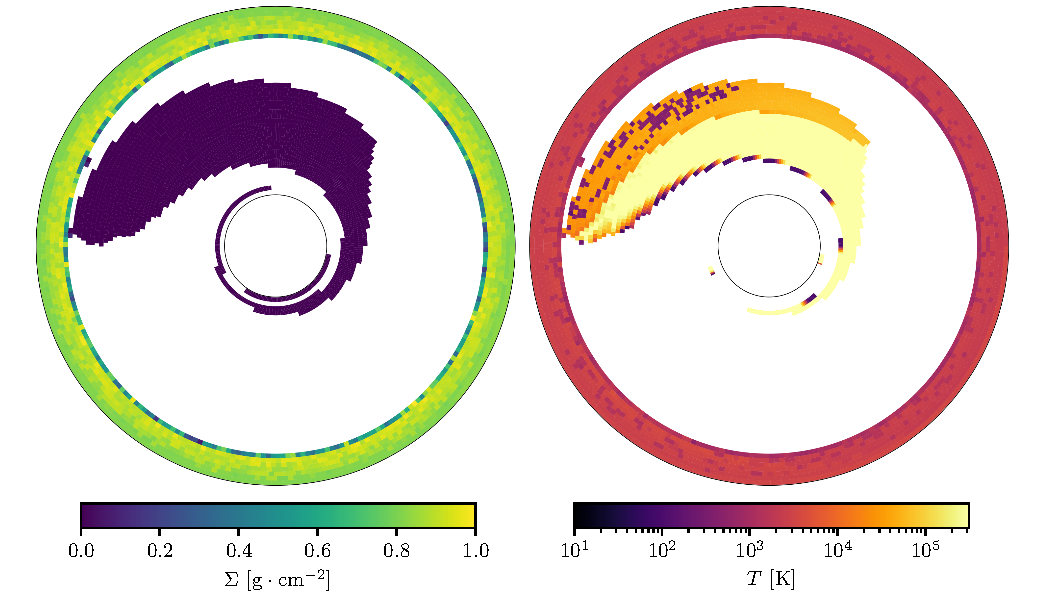
\includegraphics[width=1.0\columnwidth]{img/plot_density_temperature_c1.pdf}
        \caption{C1 ($q = 0.1$, $\psi = 0.1$) - Snapshot of the outburst from the outer stable accretion region at $7 \cdot 10^4$ steps into the SIM run.}
        \label{fig:plot_density_temperature_c1}
    \end{sidewaysfigure}

    \begin{sidewaysfigure}[h]
        \includegraphics[width=1.0\columnwidth]{img/plot_density_temperature_c2.pdf}
        \caption{C2 ($q = 0.1$, $\psi = 0.9$) - Arbitrary step in the SIM run of 2880 steps.}
        \label{fig:plot_density_temperature_c2}
    \end{sidewaysfigure}

    \begin{sidewaysfigure}[h]
        \includegraphics[width=1.0\columnwidth]{img/plot_density_temperature_c3.pdf}
        \caption{C3 ($q = 0.9$, $\psi = 0.1$) - Arbitrary step in the SIM run of 2880 steps.}
        \label{fig:plot_density_temperature_c3}
    \end{sidewaysfigure}

    \begin{sidewaysfigure}[h]
        \includegraphics[width=1.0\columnwidth]{img/plot_density_temperature_c4.pdf}
        \caption{C4 ($q = 0.9$, $\psi = 0.9$) - Arbitrary step in the SIM run of 2880 steps.}
        \label{fig:plot_density_temperature_c4}
    \end{sidewaysfigure}
    
    \begin{sidewaysfigure}[h]
        \includegraphics[width=1.0\columnwidth]{img/plot_density_temperature_c5.pdf}
        \caption{C5 ($q = 0.1$, $\psi = 0.9$) - Snapshot shortly after the blob impact in the disturbed SIM run of 2880 steps.}
        \label{fig:plot_density_temperature_c5}
    \end{sidewaysfigure}

    \begin{sidewaysfigure}[h]
        \includegraphics[width=1.0\columnwidth]{img/plot_density_temperature_c6.pdf}
        \caption{C6 ($q = 0.9$, $\psi = 0.1$) - Snapshot shortly after the blob impact in the disturbed SIM run of 2880 steps.}
        \label{fig:plot_density_temperature_c6}
    \end{sidewaysfigure}

    \begin{sidewaysfigure}[h]
        \includegraphics[width=1.0\columnwidth]{img/plot_density_temperature_c7.pdf}
        \caption{C7 ($q = 0.9$, $\psi = 0.9$) - Snapshot shortly after the blob impact in the disturbed SIM run of 2880 steps.}
        \label{fig:plot_density_temperature_c7}
    \end{sidewaysfigure}
